\documentclass[aspectratio=169]{beamer}

\usepackage{fontspec}
\usepackage[table]{xcolor}
\usepackage{amsmath,amssymb}
\usepackage{graphicx}
\usepackage{svg}
\usepackage{booktabs,array}
\usepackage{natbib}
\usepackage{tikz}
\usetikzlibrary{arrows.meta,positioning}
\bibpunct{[}{]}{,}{a}{,}{,}

\definecolor{mydarkred}{HTML}{990000}
\hypersetup{
  colorlinks=true,
  citecolor=mydarkred,
  linkcolor=black,
  urlcolor=blue
}

\usetheme{default}
\setbeamertemplate{navigation symbols}{}
\setbeamertemplate{headline}{}
\setbeamersize{text margin left=0.65cm,text margin right=0.65cm}
\setbeamerfont{title}{size=\Large}
\setbeamerfont{frametitle}{size=\large}
\setbeamerfont{framesubtitle}{size=\small}
\setbeamerfont{block title}{size=\small,series=\bfseries}
\setbeamerfont{block body}{size=\small}
\setbeamercolor{normal text}{fg=black!82,bg=white}
\setbeamercolor{frametitle}{fg=blue!55!black}
\setbeamercolor{structure}{fg=blue!55!black}
\setbeamercolor{block title}{fg=white,bg=blue!60!black}
\setbeamercolor{block body}{bg=blue!4!white}
\setbeamercolor{exampleblock title}{fg=white,bg=green!45!black}
\setbeamercolor{exampleblock body}{bg=green!5!white}
\setbeamercolor{alertblock title}{fg=white,bg=red!65!black}
\setbeamercolor{alertblock body}{bg=red!5!white}
\setbeamertemplate{footline}{\hfill\scriptsize\insertframenumber\hspace{0.65cm}\vspace{0.2cm}}

\newcommand{\takeaway}[1]{\begin{alertblock}{Thông điệp chính}#1\end{alertblock}}
\newcommand{\freeze}{\textcolor{white}{đóng băng}}
\newcommand{\update}{\textcolor{red!70!black}{cập nhật}}
\newcommand{\paperref}[1]{\textcolor{mydarkred}{[\citeauthor{#1}, \citeyear{#1}]}}
\newcommand{\step}[2]{\textbf{#1.}~#2}

\title[THESIS]{THESIS: A Robust Multi-Task Framework for Time Series Anomaly Detection with Stochastic Uncertainty}
\author[THESIS team]{Anh-Khoi Nguyen\inst{1} \and Tung Kieu\inst{2} \and Bac Le\inst{1}}
\institute[]{\inst{1} VNUHCM - University of Science\\\inst{2} Aalborg University, Denmark}
\date[Bachelor thesis defense 2026]{Bachelor thesis defense: 28th August, 2026}

\begin{document}
\setcitestyle{square,aysep={,}}

\begin{frame}\titlepage\end{frame}

\section{Mở đầu và đặt bài toán}

\begin{frame}{Bài toán cần giải quyết}
  \begin{columns}[T,onlytextwidth]
    \begin{column}{0.56\textwidth}
      \begin{block}{Hình thức hóa}
        \scriptsize
        \[
        \mathbf X_t\in\mathbb R^{L\times C},\quad
        s_{t,i}=\frac{1}{C}\lVert\mathbf x_{t,i}-\widehat{\mathbf x}_{t,i}\rVert_2^2,
        \quad \widehat a_{t,i}=\mathbb I(s_{t,i}>\delta).
        \]
        \(L\): độ dài cửa sổ; \(C\): số kênh.
      \end{block}
    \end{column}
    \begin{column}{0.40\textwidth}
      \begin{center}
        \begin{tikzpicture}[x=0.20cm,y=0.45cm,>=Latex]
          \draw[->] (0,0)--(20,0) node[right]{thời gian};
          \draw[blue!65!black,thick] plot coordinates {(0,1) (2,1.2) (4,0.9) (6,1.3) (8,1.1) (10,1.4) (12,1.2) (14,1.3) (16,3.4) (18,1.5) (20,1.4)};
          \fill[red!70!black] (16,3.4) circle (2pt);
          \node[red!70!black,above] at (16,3.4) {bất thường};
        \end{tikzpicture}
      \end{center}
      \takeaway{Phát hiện đúng cả điểm bất thường và khoảng bất thường.}
    \end{column}
  \end{columns}
\end{frame}

\begin{frame}{Bối cảnh sử dụng}
  \begin{columns}[T,onlytextwidth]
    \begin{column}{0.32\textwidth}\centering
      \includegraphics[width=\linewidth,height=0.43\textheight,keepaspectratio]{../images/semiconductor-equipment-process.png}\\[-0.15em]
      \small Sản xuất bán dẫn\\[-0.15em]
      \paperref{kim2026sacvt}
    \end{column}
    \begin{column}{0.32\textwidth}\centering
      
\includegraphics[width=\linewidth,height=0.43\textheight,keepaspectratio]{../images/cloud-systems-log.jpg}\\[-0.15em]
      \small Giám sát hệ thống đám mây\\[-0.15em]
      \paperref{11121677}
    \end{column}
    \begin{column}{0.32\textwidth}\centering
      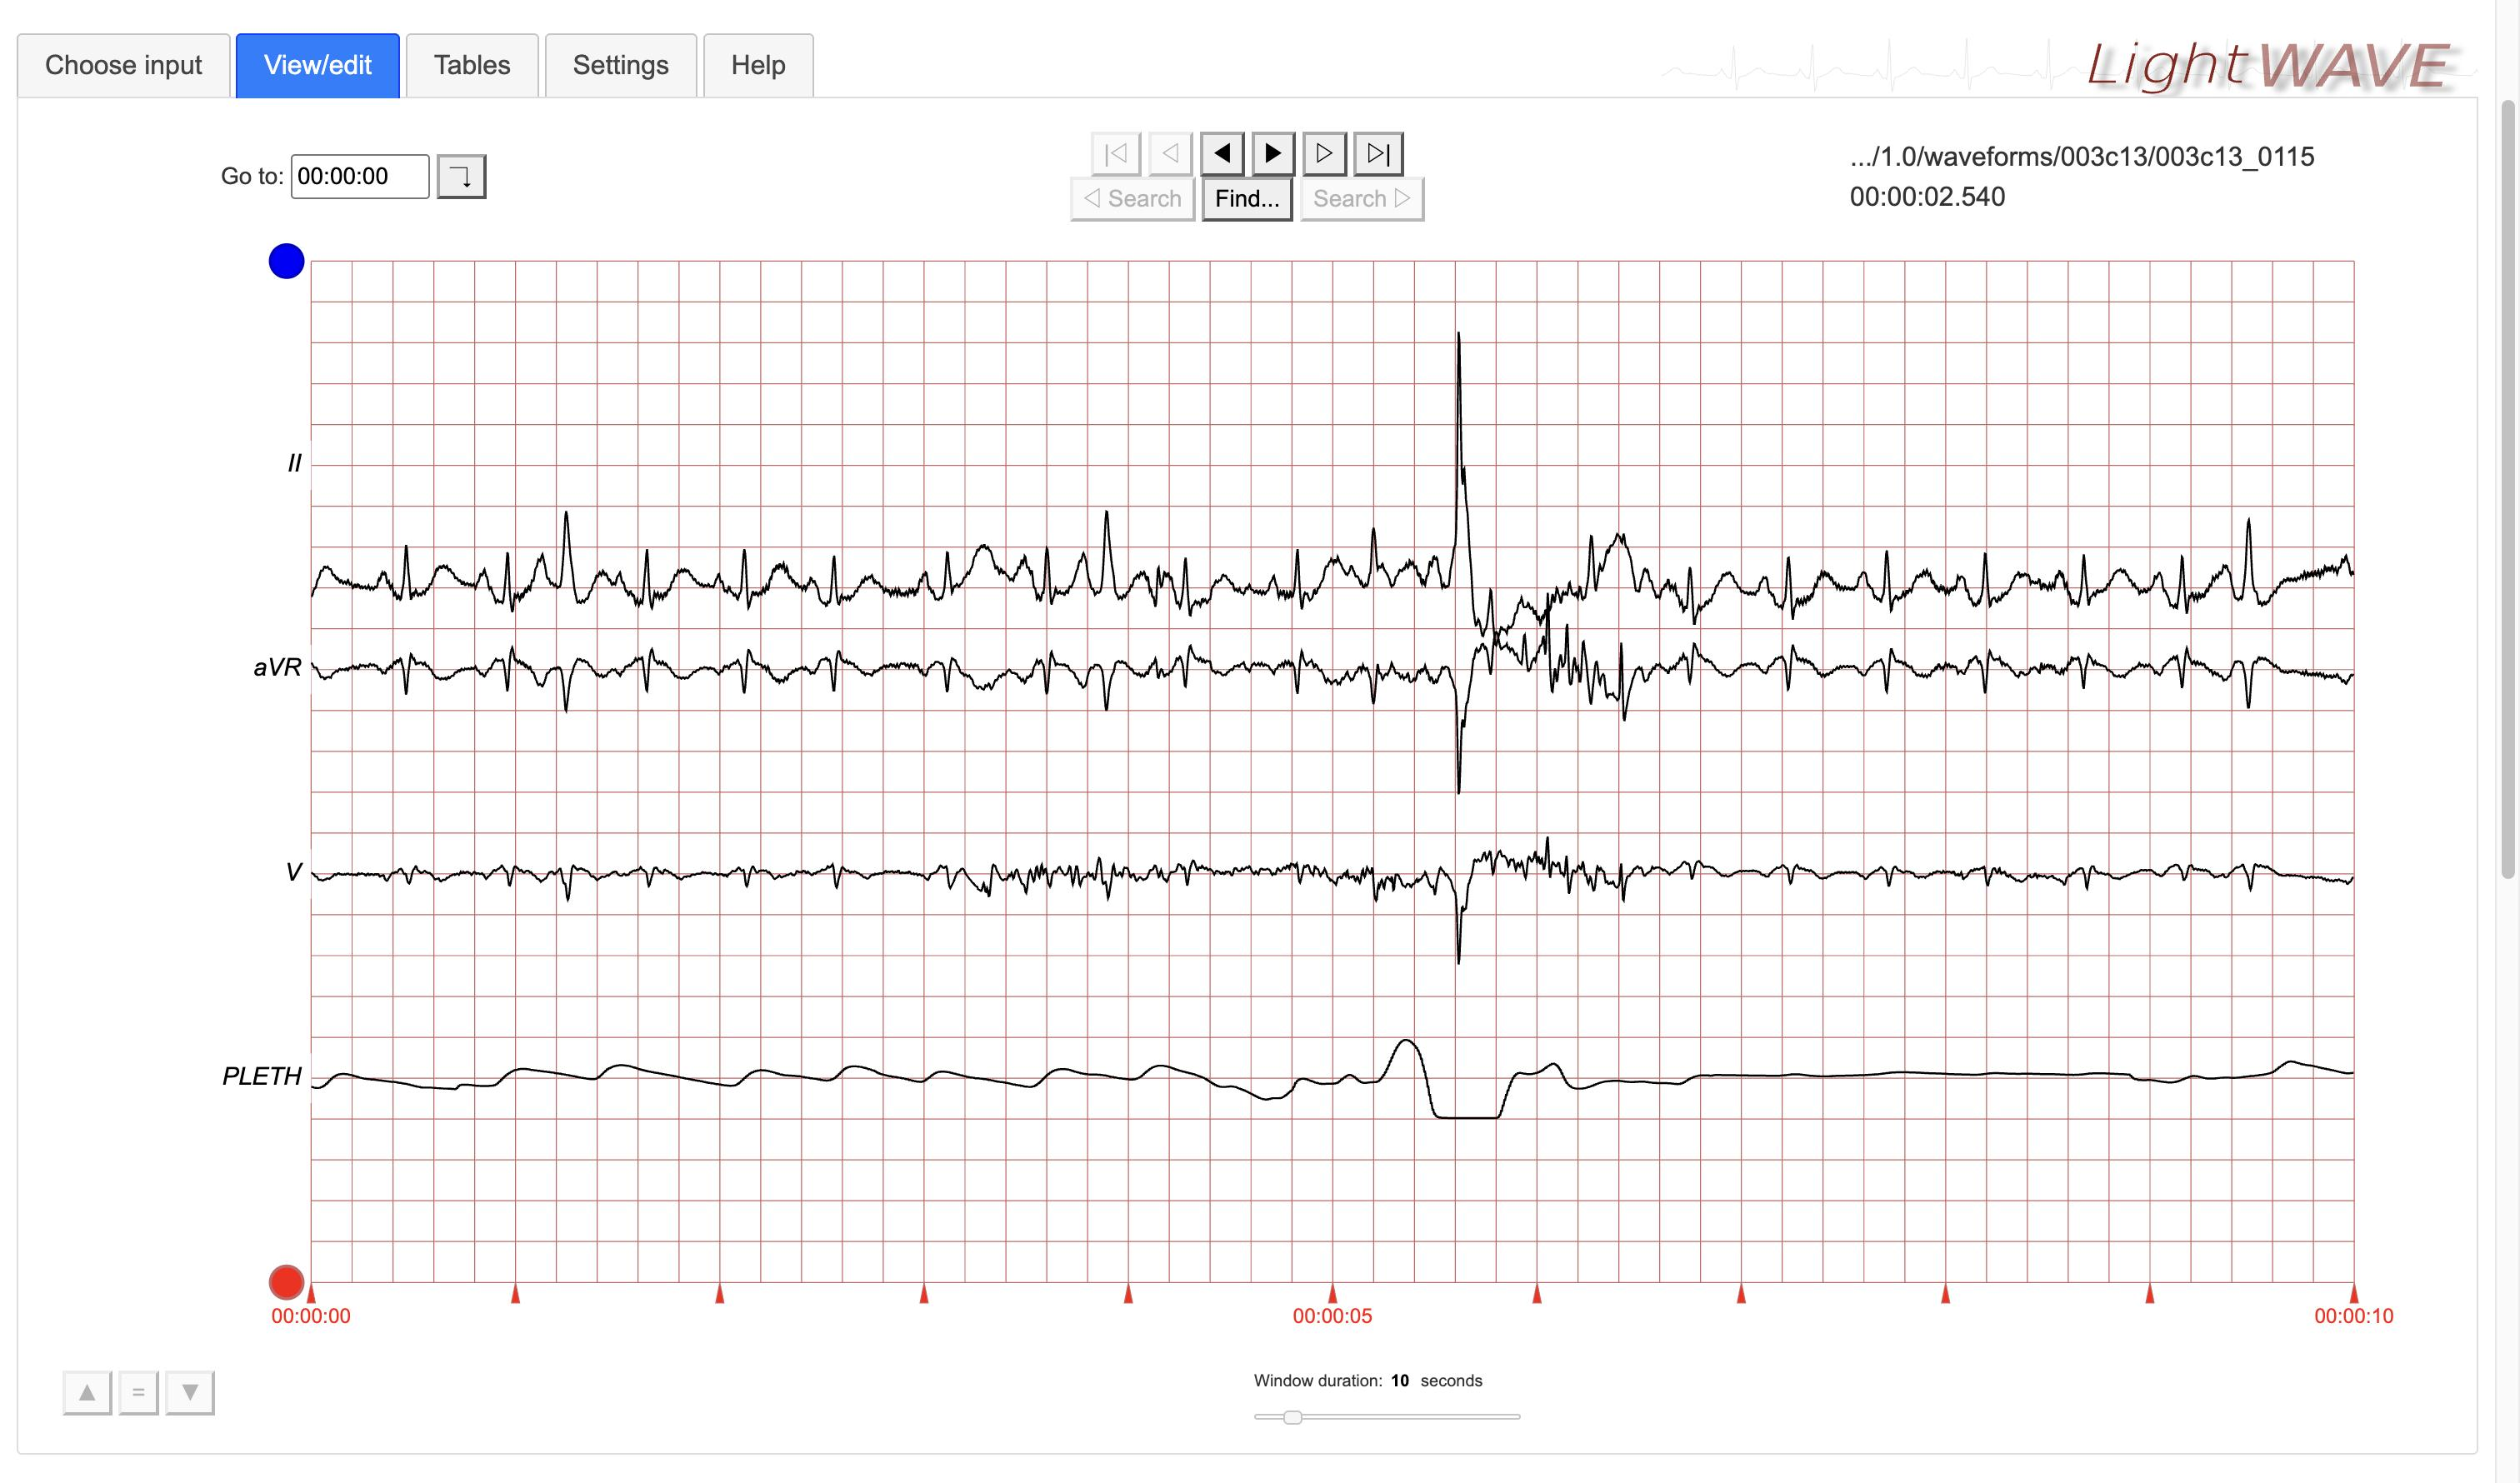
\includegraphics[width=\linewidth,height=0.43\textheight,keepaspectratio]{../images/icu-vital-signs.jpg}\\[-0.15em]
      \small Theo dõi dấu hiệu sinh tồn\\[-0.15em]
      \paperref{PhysioNet-vtac-1.0}
    \end{column}
  \end{columns}
  \takeaway{Báo động sai có thể làm tăng chi phí và gây mệt mỏi vì báo động.}
\end{frame}

\begin{frame}{Hai hạn chế cần xử lý}
  \begin{columns}[T,onlytextwidth]
    \begin{column}{0.48\textwidth}\begin{alertblock}{Quá tự tin}Mạng nơ-ron có thể cho điểm số chắc chắn khi dữ liệu mới khác phân phối huấn luyện.\end{alertblock}\end{column}
    \begin{column}{0.48\textwidth}\begin{alertblock}{Khó thích ứng}Dòng dữ liệu không dừng làm giảm chất lượng nếu mô hình không được cập nhật có kiểm soát.\end{alertblock}\end{column}
  \end{columns}
  \takeaway{Cần đo độ bất định và thích ứng, nhưng không được học nhầm bất thường.}
\end{frame}

\begin{frame}{Các công trình liên quan}
  \scriptsize
  \begin{tabular}{>{\raggedright\arraybackslash}p{0.27\linewidth} >{\raggedright\arraybackslash}p{0.67\linewidth}}
    \toprule
    Công trình & Vai trò trong khóa luận \\
    \midrule
    \paperref{redlamp2025} & Nền cho khung huấn luyện đa tác vụ. \\
    \paperref{shen2025learn} & Bộ nhớ và truy vấn liên tục được kế thừa. \\
    \paperref{oord2017neural} & Bộ nhớ và truy vấn rời rạc được kế thừa. \\
    \paperref{zhang2024adarealign} & Cảm hứng cho việc kéo biểu diễn trực tuyến về nhánh nguồn. \\
    \paperref{pei2022transformer} & Cảm hứng cho nhiễu Gumbel trong ma trận tương đồng. \\
    \bottomrule
  \end{tabular}
  \takeaway{Khóa luận kế thừa từng thành phần và đề xuất cách phối hợp chúng trong một luồng đa nhiệm.}
\end{frame}

\section{Tính mới và kiến trúc đề xuất}

\begin{frame}{Ranh giới giữa kế thừa và đề xuất mới}
  \begin{columns}[T,onlytextwidth]
    \begin{column}{0.47\textwidth}\begin{block}{Dùng làm nền}Bộ mã hóa dùng chung; đầu tái tạo; đầu phân loại; K-Means; các họ bất thường nhân tạo; VUS-PR và Affiliation F1-score.\end{block}\end{column}
    \begin{column}{0.47\textwidth}\begin{exampleblock}{Phần đề xuất hoặc phối hợp}Hai toán tử truy vấn; hai phiên bản ngẫu nhiên; thích ứng trực tuyến; quy tắc tam phân; bộ đệm xác minh.\end{exampleblock}\end{column}
  \end{columns}
  \takeaway{Tính mới nằm ở thiết kế khung và chính sách vận hành, không phải ở mọi thành phần riêng lẻ.}
\end{frame}

\begin{frame}{Kiến trúc tổng quát của pha ngoại tuyến}
  \begin{center}
    \includesvg[inkscapelatex=false,width=0.94\linewidth]{../images/architecture-thesis.drawio}
  \end{center}
  \takeaway{Một bộ mã hóa dùng chung tạo biểu diễn cho tái tạo và phân loại qua hai bộ nhớ.}
\end{frame}

\begin{frame}{Bốn hoạt động chính của toàn hệ thống}
  \small
  \begin{tabular}{>{\raggedright\arraybackslash}p{0.22\linewidth} p{0.34\linewidth} p{0.34\linewidth}}
    \toprule
    & Huấn luyện & Suy luận \\
    \midrule
    Ngoại tuyến & Học biểu diễn; khởi tạo bộ nhớ; tinh chỉnh đầu ra. & Hiệu chỉnh ngưỡng trên xác thực sạch; đánh giá kiểm tra. \\
    Trực tuyến & Cập nhật có điều kiện chỉ bộ ánh xạ trực tuyến. & Cửa sổ mới → điểm số → làm trơn → dự đoán → quyết định cập nhật. \\
    \bottomrule
  \end{tabular}
  \takeaway{Huấn luyện và suy luận là hai hoạt động khác nhau ở cả hai pha.}
\end{frame}

\section{Luồng dữ liệu của pha ngoại tuyến}

\begin{frame}{Luồng chuẩn bị dữ liệu ngoại tuyến}
  \begin{center}
    \begin{tikzpicture}[node distance=0.35cm,>=Latex]
      \tikzset{box/.style={draw,rounded corners,align=center,minimum width=2.2cm,minimum height=0.9cm,fill=blue!5}}
      \node[box] (raw) {Chuỗi gốc};\node[box,right=of raw] (scale) {Chuẩn hóa\\theo tập huấn luyện};\node[box,right=of scale] (window) {Cửa sổ\\$20\times38$};\node[box,right=of window] (batch) {Lô\\$B\times20\times38$};
      \draw[->,thick] (raw)--(scale);\draw[->,thick] (scale)--(window);\draw[->,thick] (window)--(batch);
    \end{tikzpicture}
  \end{center}
  \begin{columns}[T,onlytextwidth]
    \begin{column}{0.48\textwidth}\begin{block}{Thống kê}Trung bình và độ lệch chuẩn chỉ được tính trên tập huấn luyện.\end{block}\end{column}
    \begin{column}{0.48\textwidth}\begin{block}{Sử dụng lại}Xác thực và kiểm tra dùng cùng thống kê, không học lại bộ chuẩn hóa.\end{block}\end{column}
  \end{columns}
\end{frame}

\begin{frame}{Vị trí tiêm bất thường nhân tạo}
  \begin{center}
    \begin{tikzpicture}[node distance=0.25cm,>=Latex]
      \tikzset{box/.style={draw,rounded corners,align=center,minimum width=2.1cm,minimum height=0.8cm}}
      \node[box] (clean) {Lô cửa sổ sạch};\node[box,right=of clean,fill=orange!15] (inject) {Tiêm bất thường};\node[box,right=of inject] (encode) {Bộ mã hóa};\node[box,right=of encode] (heads) {Các đầu ra};
      \draw[->,thick] (clean)--(inject);\draw[->,thick] (inject)--(encode);\draw[->,thick] (encode)--(heads);
    \end{tikzpicture}
  \end{center}
  \begin{columns}[T,onlytextwidth]
    \begin{column}{0.48\textwidth}\begin{block}{Đầu ra của bộ tiêm}Cửa sổ đã thay đổi, nhãn lớp, mặt nạ điểm và siêu dữ liệu.\end{block}\end{column}
    \begin{column}{0.48\textwidth}\begin{alertblock}{Ranh giới}Đây là bước tạo dữ liệu huấn luyện; pha trực tuyến không gọi bộ tiêm.\end{alertblock}\end{column}
  \end{columns}
\end{frame}

\begin{frame}{Mã nguồn tiêm bất thường làm gì?}
  \scriptsize
  \begin{columns}[T,onlytextwidth]
    \begin{column}{0.52\textwidth}
      \begin{block}{Cấu hình thực tế}
        \setlength{\tabcolsep}{2pt}
        \begin{tabular}{ll}
          Lớp dữ liệu & 1 bình thường + 11 bất thường \\
          Đoạn liên tục & 20\%–30\% cửa sổ \\
          Với $L=20$ & thường 4–6 điểm \\
          Kênh bị thay đổi & 10\%–50\% số kênh \\
          Với $C=38$ & khoảng 3–19 kênh \\
          Cân bằng lớp & 12 lớp gần đều trong lô \\
        \end{tabular}
      \end{block}
    \end{column}
    \begin{column}{0.43\textwidth}
      \begin{exampleblock}{11 họ bất thường}
        Tăng đột ngột; lật; tăng nhịp độ; nhiễu; cắt theo ngưỡng; trung bình hóa; co giãn; dao động trôi dạt; theo ngữ cảnh; lật dọc; hỗn hợp.
      \end{exampleblock}
      \begin{center}
        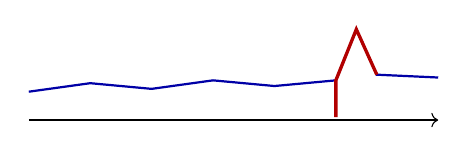
\begin{tikzpicture}[x=0.26cm,y=0.36cm]
          \draw[->] (0,0)--(20,0);
          \draw[blue!65!black,thick] plot coordinates {(0,1) (3,1.3) (6,1.1) (9,1.4) (12,1.2) (15,1.4) (16,3.2) (17,1.6) (20,1.5)};
          \draw[red!70!black,very thick] (15,0.1)--(15,1.4)--(16,3.2)--(17,1.6);
        \end{tikzpicture}
      \end{center}
    \end{column}
  \end{columns}
  \takeaway{Mặt nạ đánh dấu đúng vị trí bị thay đổi.}
\end{frame}

\begin{frame}{Giai đoạn học biểu diễn đa nhiệm}
  \begin{columns}[T,onlytextwidth]
    \begin{column}{0.58\textwidth}\includesvg[inkscapelatex=false,width=\linewidth]{../images/pretrain-stage-arch.drawio}\end{column}
    \begin{column}{0.38\textwidth}
      \begin{block}{Mục tiêu}
        \[
        \mathcal L_A=\lambda_{\rm rec}\mathcal L_{\rm rec}+\lambda_{\rm cls}\mathcal L_{\rm cls}+\lambda_{\rm con}\mathcal L_{\rm con}.
        \]
        Tái tạo, phân loại 12 lớp và học tương phản.
      \end{block}
      \begin{exampleblock}{Cấu hình}25 vòng lặp huấn luyện.\end{exampleblock}
    \end{column}
  \end{columns}
  \takeaway{Bất thường nhân tạo tạo tín hiệu giám sát cho biểu diễn.}
\end{frame}

\begin{frame}{Khởi tạo hai bộ nhớ}
  \begin{center}
    \begin{tikzpicture}[node distance=0.45cm,>=Latex]
      \tikzset{box/.style={draw,rounded corners,align=center,minimum width=2.7cm,minimum height=0.85cm}}
      \node[box] (z) {Biểu diễn ẩn\\sau giai đoạn A};\node[box,below left=0.55cm and 0.2cm of z,fill=blue!10] (pc) {K-Means\\32 nguyên mẫu liên tục};\node[box,below right=0.55cm and 0.2cm of z,fill=orange!15] (pd) {12 lớp × 5\\60 mã rời rạc};
      \draw[->,thick] (z)--(pc);\draw[->,thick] (z)--(pd);
    \end{tikzpicture}
  \end{center}
  \takeaway{Hai bộ nhớ lấy từ cùng biểu diễn đã học và được đóng băng trước khi tinh chỉnh.}
\end{frame}

\begin{frame}{Giai đoạn tinh chỉnh mạng tổng hợp}
  \begin{columns}[T,onlytextwidth]
    \begin{column}{0.58\textwidth}\includesvg[inkscapelatex=false,width=\linewidth]{../images/fine-tune-stage-arch.drawio}\end{column}
    \begin{column}{0.38\textwidth}
      \begin{block}{\freeze}Bộ mã hóa và hai bộ nhớ.\end{block}
      \begin{alertblock}{\update}Các mạng tổng hợp và đầu dự đoán.\end{alertblock}
      \begin{exampleblock}{Cấu hình}5 vòng lặp huấn luyện.\end{exampleblock}
    \end{column}
  \end{columns}
  \takeaway{Giai đoạn B học cách kết hợp biểu diễn gốc với hai biểu diễn truy vấn.}
\end{frame}

\section{Các toán tử truy vấn và độ bất định}

\begin{frame}{Biểu diễn ẩn và hai bộ nhớ}
  \begin{columns}[T,onlytextwidth]
    \begin{column}{0.46\textwidth}\begin{block}{Biểu diễn}\[\mathbf Z=f_{\rm enc}(\mathbf X)\in\mathbb R^{L\times H},\qquad \lVert\mathbf z_i\rVert_2=1.\]\end{block}\end{column}
    \begin{column}{0.46\textwidth}\begin{block}{Bộ nhớ}\(P^{(c)}\): 32 nguyên mẫu liên tục.\\\(P^{(d)}\): 60 mã rời rạc thuộc 12 lớp.\end{block}\end{column}
  \end{columns}
  \begin{center}
    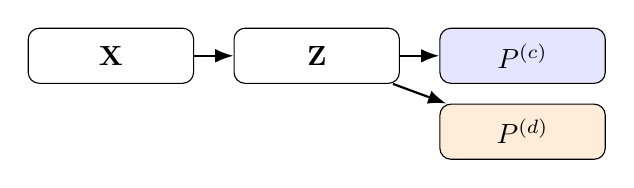
\begin{tikzpicture}[node distance=0.5cm,>=Latex]
      \tikzset{box/.style={draw,rounded corners,minimum width=2.1cm,minimum height=0.7cm,align=center}}
      \node[box] (x) {$\mathbf X$};\node[box,right=of x] (z) {$\mathbf Z$};\node[box,right=of z,fill=blue!10] (c) {$P^{(c)}$};\node[box,below=0.25cm of c,fill=orange!15] (d) {$P^{(d)}$};
      \draw[->,thick] (x)--(z);\draw[->,thick] (z)--(c);\draw[->,thick] (z)--(d);
    \end{tikzpicture}
  \end{center}
\end{frame}

\begin{frame}{Truy vấn liên tục xác định}
  \begin{columns}[T,onlytextwidth]
    \begin{column}{0.47\textwidth}\begin{block}{Gán trọng số}\[\alpha^{(c)}_{i,k}=\operatorname{softmax}_k\left(\frac{\mathbf z_i^\mathsf T\mathbf p_k^{(c)}}{\tau_c}\right).\]\small Độ tương đồng cao thì trọng số lớn.\end{block}\end{column}
    \begin{column}{0.47\textwidth}\begin{exampleblock}{Biểu diễn truy vấn}\[\widetilde{\mathbf z}^{(c)}_i=\sum_{k=1}^{K_c}\alpha^{(c)}_{i,k}\mathbf p_k^{(c)}.\]\small Tất cả 32 nguyên mẫu đều có thể đóng góp.\end{exampleblock}\end{column}
  \end{columns}
  \takeaway{Truy vấn liên tục là truy vấn dày.}
\end{frame}

\begin{frame}{Truy vấn rời rạc xác định}
  \begin{columns}[T,onlytextwidth]
    \begin{column}{0.48\textwidth}\begin{block}{Chọn lân cận}\[\begin{aligned} d^{(d)}_{i,k}&=\lVert\mathbf z_i-\mathbf p_k^{(d)}\rVert_2^2,\\ \mathcal I_i&=\operatorname{TopKMin}_k(d^{(d)}_{i,k};3). \end{aligned}\]\end{block}\end{column}
    \begin{column}{0.46\textwidth}\begin{exampleblock}{Truy xuất}\[\widetilde{\mathbf z}^{(d)}_i=\sum_{k\in\mathcal I_i}\alpha^{(d)}_{i,k}\mathbf p_k^{(d)}.\]\small Chỉ ba mã gần nhất đóng góp.\end{exampleblock}\end{column}
  \end{columns}
  \takeaway{Truy vấn rời rạc là truy vấn thưa.}
\end{frame}

\begin{frame}{Truy vấn liên tục ngẫu nhiên}
  \begin{columns}[T,onlytextwidth]
    \begin{column}{0.48\textwidth}\begin{block}{Thêm nhiễu}\[\begin{aligned} g^{(c,m)}_{i,k}&\sim\operatorname{Gumbel}(0,1),\\ \alpha^{(c,m)}_{i,k}&=\operatorname{softmax}_k\left(\frac{\mathbf z_i^\mathsf T\mathbf p_k^{(c)}+g^{(c,m)}_{i,k}}{\tau_c}\right). \end{aligned}\]\end{block}\end{column}
    \begin{column}{0.46\textwidth}\begin{exampleblock}{Mỗi lượt truy vấn}\[\widetilde{\mathbf z}^{(c,m)}_i=\sum_k\alpha^{(c,m)}_{i,k}\mathbf p_k^{(c)}.\]\small Nhiều lượt tạo nhiều hỗn hợp liên tục khác nhau.\end{exampleblock}\end{column}
  \end{columns}
  \takeaway{Độ bất định đến từ sự thay đổi giữa các lượt truy vấn.}
\end{frame}

\begin{frame}{Truy vấn rời rạc ngẫu nhiên}
  \begin{columns}[T,onlytextwidth]
    \begin{column}{0.48\textwidth}\begin{block}{Chọn lại lân cận}\[\begin{aligned} q^{(d,m)}_{i,k}&=\frac{-d^{(d)}_{i,k}+g^{(d,m)}_{i,k}}{\tau_d},\\ \mathcal I_i^{(d,m)}&=\operatorname{TopKMax}_k(q^{(d,m)}_{i,k};3). \end{aligned}\]\end{block}\end{column}
    \begin{column}{0.46\textwidth}\begin{exampleblock}{Kết quả}\[\widetilde{\mathbf z}^{(d,m)}_i=\sum_{k\in\mathcal I_i^{(d,m)}}\alpha^{(d,m)}_{i,k}\mathbf p_k^{(d)}.\]\small Lân cận ba mã có thể đổi theo lượt \(m\).\end{exampleblock}\end{column}
  \end{columns}
  \takeaway{Độ bất định đến từ cả trọng số và tập mã được chọn.}
\end{frame}

\begin{frame}{Tính độ bất định}
  \begin{columns}[T,onlytextwidth]
    \begin{column}{0.48\textwidth}\begin{block}{Luồng tính}\step{1}{Giữ bộ mã hóa nguồn cố định.}\\\step{2}{Lấy nhiễu mới cho mỗi lượt.}\\\step{3}{Tạo \(\widehat{\mathbf X}^{(m)}\) và \(s_i^{(m)}\).}\\\step{4}{Lặp \(M=10\) lượt.}\end{block}\end{column}
    \begin{column}{0.48\textwidth}\begin{exampleblock}{Hai đại lượng}\[\begin{aligned} \overline{s}_i&=\frac1M\sum_{m=1}^M s_i^{(m)},\\ u_i^2&=\frac1{M-1}\sum_{m=1}^M(s_i^{(m)}-\overline{s}_i)^2. \end{aligned}\]\(\overline s_i\) dùng dự đoán; \(u_i^2\) dùng chẩn đoán.\end{exampleblock}\end{column}
  \end{columns}
  \takeaway{Độ bất định cao không tự động có nghĩa là điểm đó bất thường.}
\end{frame}

\begin{frame}{Suy luận ngoại tuyến và hiệu chỉnh ngưỡng}
  \begin{center}
    \begin{tikzpicture}[node distance=0.25cm,>=Latex]
      \tikzset{box/.style={draw,rounded corners,align=center,minimum width=2.15cm,minimum height=0.8cm}}
      \node[box] (model) {Mô hình tốt nhất};\node[box,right=of model] (val) {Xác thực sạch\\không chồng lấp};\node[box,right=of val] (score) {Điểm tái tạo};\node[box,right=of score,fill=orange!15] (th) {Chọn ngưỡng};\node[box,right=of th] (test) {Kiểm tra};
      \foreach \a/\b in {model/val,val/score,score/th,th/test}{\draw[->,thick] (\a)--(\b);}
    \end{tikzpicture}
  \end{center}
  \begin{columns}[T,onlytextwidth]
    \begin{column}{0.48\textwidth}\begin{block}{Được dùng}\small Chỉ xác thực sạch để chọn ngưỡng.\end{block}\end{column}
    \begin{column}{0.48\textwidth}\begin{alertblock}{Không được dùng}\small Không dùng nhãn kiểm tra để chọn ngưỡng.\end{alertblock}\end{column}
  \end{columns}
  \takeaway{Ngưỡng được cố định trước khi đánh giá tập kiểm tra.}
\end{frame}

\section{Luồng dữ liệu của pha trực tuyến}

\begin{frame}{Kiến trúc và dữ liệu đầu vào trực tuyến}
  \begin{columns}[T,onlytextwidth]
    \begin{column}{0.60\textwidth}\includesvg[inkscapelatex=false,width=\linewidth]{../images/online-adaptation-arch.drawio}\end{column}
    \begin{column}{0.36\textwidth}\begin{block}{\freeze}Bộ mã hóa, hai bộ nhớ, mạng tổng hợp và đầu dự đoán.\end{block}\begin{alertblock}{\update}Chỉ bộ ánh xạ trực tuyến.\end{alertblock}\end{column}
  \end{columns}
  \takeaway{Pha trực tuyến tái sử dụng mô hình ngoại tuyến và chỉ mở một vùng tham số nhỏ.}
\end{frame}

\begin{frame}{Từ dữ liệu thô đến điểm dự đoán}
  \scriptsize
  \begin{center}
    \begin{tikzpicture}[node distance=0.16cm,>=Latex]
      \tikzset{box/.style={draw,rounded corners,align=center,minimum width=1.65cm,minimum height=0.58cm,fill=blue!4}}
      \node[box] (a) {1. Điểm mới};\node[box,right=of a] (b) {2. Chuẩn hóa};\node[box,right=of b] (c) {3. Cửa sổ trượt};\node[box,right=of c] (d) {4. Biểu diễn nguồn};\node[box,right=of d] (e) {5. Ánh xạ trực tuyến};
      \node[box,below=0.35cm of c,fill=orange!12] (f) {6. Truy vấn ngẫu nhiên, $M=10$};\node[box,right=of f] (g) {7. Tái tạo};\node[box,right=of g] (h) {8. Điểm trung bình};\node[box,right=of h] (i) {9. Ghép chỉ số};
      \node[box,below=0.35cm of g,fill=green!10] (j) {10. EWMA, $\rho=0.9$};\node[box,right=of j] (k) {11. Ngưỡng → nhãn};
      \foreach \a/\b in {a/b,b/c,c/d,d/e,e/f,f/g,g/h,h/i,i/j,j/k}{\draw[->,thick] (\a)--(\b);}
    \end{tikzpicture}
  \end{center}
  \begin{center}\small Pha trực tuyến không gọi bộ tiêm bất thường nhân tạo.\end{center}
  \takeaway{Dữ liệu thô chỉ trở thành quyết định sau khi đi qua toàn bộ chuỗi xử lý.}
\end{frame}

\begin{frame}{Điểm số và quyết định ở hai mức}
  \begin{columns}[T,onlytextwidth]
    \begin{column}{0.47\textwidth}\begin{block}{Mức điểm thời gian}\[\widehat a_n=\mathbb I(\widetilde s_n>\delta_{\rm pt}).\]Một điểm được gắn nhãn bất thường khi điểm đã làm trơn vượt ngưỡng.\end{block}\end{column}
    \begin{column}{0.47\textwidth}\begin{exampleblock}{Mức cửa sổ}Dùng trung bình điểm trong cửa sổ và khoảng cách ẩn đến nguyên mẫu liên tục để phân luồng.\end{exampleblock}\end{column}
  \end{columns}
  \takeaway{Điểm thời gian tạo nhãn; cửa sổ tạo quyết định có nên cập nhật hay không.}
\end{frame}

\begin{frame}{Quy tắc tam phân và bộ đệm xác minh}
  \scriptsize
  \begin{tabular}{>{\raggedright\arraybackslash}p{0.23\linewidth} >{\raggedright\arraybackslash}p{0.46\linewidth} >{\raggedright\arraybackslash}p{0.20\linewidth}}
    \toprule
    Luồng & Điều kiện và diễn giải & Hành động \\
    \midrule
    Bình thường & Sai số cửa sổ không vượt ngưỡng. & Bỏ qua \\
    Bình thường khó & Sai số cao nhưng biểu diễn gần mẫu bình thường đã lưu. & Cập nhật có điều kiện \\
    Vùng xám & Sai số cao, chưa đủ bằng chứng. & Đưa vào bộ đệm \\
    Bất thường mạnh & Sai số cao và biểu diễn xa mẫu bình thường. & Không cập nhật \\
    \bottomrule
  \end{tabular}
  \begin{center}\small Ba trường hợp cần xử lý khi sai số cửa sổ cao: bình thường khó, vùng xám, bất thường mạnh.\end{center}
  \takeaway{Tam phân sàng lọc nhanh; bộ đệm xác minh kiểm tra vùng chưa chắc chắn.}
\end{frame}

\begin{frame}{Vì sao không gộp hai bước?}
  \begin{columns}[T,onlytextwidth]
    \begin{column}{0.47\textwidth}\begin{block}{Quy tắc tam phân}Tính rẻ trên từng cửa sổ. Nó tách mẫu rõ ràng để giảm số cửa sổ phải xử lý sâu.\end{block}\end{column}
    \begin{column}{0.47\textwidth}\begin{alertblock}{Bộ đệm xác minh}Giữ các cửa sổ vùng xám không chồng lấp, kiểm tra lặp lại mẫu hình rồi mới cập nhật.\end{alertblock}\end{column}
  \end{columns}
  \takeaway{Gộp hai bước sẽ hoặc tốn chi phí trên mọi cửa sổ, hoặc dễ cập nhật nhầm bất thường.}
\end{frame}

\begin{frame}{Hàm mất mát tương phản trực tuyến}
  \begin{columns}[T,onlytextwidth]
    \begin{column}{0.48\textwidth}\begin{block}{Mục tiêu}Kéo biểu diễn trực tuyến gần biểu diễn nguồn trên cùng cửa sổ; đẩy xa các nguyên mẫu bất thường.\[\mathcal L_{\rm on}=\mathcal L_{\rm hard-rec}+\lambda\mathcal L_{\rm src-on}.\]\end{block}\end{column}
    \begin{column}{0.46\textwidth}\begin{alertblock}{Giới hạn cập nhật}Chỉ bộ ánh xạ MLP trực tuyến được cập nhật. Các mô-đun còn lại bị đóng băng.\end{alertblock}\end{column}
  \end{columns}
  \takeaway{Thích ứng có điều kiện nhằm học bình thường mới, không học mẫu bất thường.}
\end{frame}

\section{Độ đo và thiết kế thí nghiệm}

\begin{frame}{Cách tính VUS-PR}
  \begin{columns}[T,onlytextwidth]
    \begin{column}{0.48\textwidth}\begin{block}{Các bước}\step{1}{Ghép điểm số và nhãn theo thời gian.}\\\step{2}{Quét nhiều ngưỡng.}\\\step{3}{Tính precision và recall có xét vùng bất thường.}\\\step{4}{Tính diện tích dưới đường PR.}\\\step{5}{Lặp theo kích thước vùng đệm và lấy trung bình.}\end{block}\end{column}
    \begin{column}{0.46\textwidth}\begin{exampleblock}{Ý nghĩa}VUS-PR đánh giá thứ hạng điểm số khi bất thường có dạng đoạn liên tục. Trong mã nguồn hiện tại: vùng đệm 20, 200 ngưỡng.\end{exampleblock}\end{column}
  \end{columns}
  \takeaway{VUS-PR không phải là một phép đo tại một ngưỡng duy nhất.}
\end{frame}

\begin{frame}{Cách tính Affiliation F1-score}
  \begin{columns}[T,onlytextwidth]
    \begin{column}{0.48\textwidth}\begin{block}{Các bước}\step{1}{Đổi các điểm dương liên tiếp thành các sự kiện.}\\\step{2}{Đo mức giao giữa sự kiện dự đoán và sự kiện thật.}\\\step{3}{Tính precision theo vùng và recall theo vùng.}\\\step{4}{Lấy trung bình điều hòa.}\end{block}\end{column}
    \begin{column}{0.46\textwidth}\begin{exampleblock}{Công thức cuối}\[F1_{\rm aff}=\frac{2P_{\rm aff}R_{\rm aff}}{P_{\rm aff}+R_{\rm aff}}.\]Độ đo này quan tâm sự kiện và mức bao phủ của đoạn bất thường.\end{exampleblock}\end{column}
  \end{columns}
  \takeaway{Affiliation F1-score bổ sung cho VUS-PR bằng góc nhìn theo sự kiện.}
\end{frame}

\begin{frame}{Bối cảnh dữ liệu thí nghiệm}
  \scriptsize
  \begin{tabular}{lrrrr}
    \toprule
    Chuỗi SMD & Huấn luyện & Xác thực & Kiểm tra & Tổng \\
    \midrule
    Machine-1-6 & 18\,932 & 236 & 1\,184 & 20\,352 \\
    Machine-3-4 & 18\,931 & 236 & 1\,184 & 20\,351 \\
    Machine-3-9 & 22\,952 & 287 & 1\,435 & 24\,674 \\
    \bottomrule
  \end{tabular}
  \vspace{0.4em}
  \begin{columns}[T,onlytextwidth]
    \begin{column}{0.48\textwidth}\begin{block}{Cấu hình}\small Cửa sổ dài 20; 38 kênh; 3 hạt giống; 25 + 5 vòng lặp ngoại tuyến.\end{block}\end{column}
    \begin{column}{0.48\textwidth}\begin{block}{Chia dữ liệu}\small Cửa sổ xác thực ngoại tuyến không chồng lấp; cửa sổ trực tuyến dùng bước trượt 1.\end{block}\end{column}
  \end{columns}
\end{frame}

\begin{frame}{Vì sao chọn ba chuỗi này?}
  \begin{columns}[T,onlytextwidth]
    \begin{column}{0.31\textwidth}\begin{block}{Machine-1-6}\centering Có chuyển dịch phân phối giữa huấn luyện và kiểm tra.\end{block}\end{column}
    \begin{column}{0.31\textwidth}\begin{block}{Machine-3-4}\centering Có chuyển dịch đủ rõ để kiểm tra khả năng thích ứng.\end{block}\end{column}
    \begin{column}{0.31\textwidth}\begin{block}{Machine-3-9}\centering Bổ sung một chuỗi có quy mô cửa sổ khác.\end{block}\end{column}
  \end{columns}
  \takeaway{Ba chuỗi được chọn vì có chuyển dịch phân phối đáng chú ý, không phải vì đại diện cho toàn bộ SMD.}
\end{frame}

\begin{frame}{Vì sao phạm vi dữ liệu còn nhỏ?}
  \begin{columns}[T,onlytextwidth]
    \begin{column}{0.31\textwidth}\begin{alertblock}{Chi phí}\centering Huấn luyện hai giai đoạn và nhiều lượt ngẫu nhiên tốn tài nguyên.\end{alertblock}\end{column}
    \begin{column}{0.31\textwidth}\begin{alertblock}{Độ phức tạp}\centering Luồng trực tuyến có nhiều trạng thái và cần kiểm tra nguyên nhân.\end{alertblock}\end{column}
    \begin{column}{0.31\textwidth}\begin{alertblock}{Giới hạn kết luận}\centering Ba chuỗi chưa đủ để khẳng định khả năng khái quát hóa rộng.\end{alertblock}\end{column}
  \end{columns}
  \takeaway{Ít dữ liệu là giới hạn của bằng chứng, không phải bằng chứng phương pháp luôn hoạt động tốt.}
\end{frame}

\section{Kết quả, FPR và kết luận}

\begin{frame}{Kết quả pha ngoại tuyến}
  \scriptsize
  \begin{tabular}{lccc}
    \toprule
    Phương pháp & VUS-PR & Affiliation F1 & VUS-ROC \\
    \midrule
    \textbf{THESIS O0} & \textbf{0.694} & 0.748 & 0.829 \\
    \textbf{THESIS O1} & \textbf{0.694} & \textbf{0.749} & 0.829 \\
    RedLamp & 0.573 & 0.744 & 0.646 \\
    iForest & 0.149 & 0.410 & 0.568 \\
    KMeans-AD & 0.455 & 0.379 & \textbf{0.872} \\
    \bottomrule
  \end{tabular}
  \begin{exampleblock}{Diễn giải}THESIS có kết quả trung bình tốt trên VUS-PR và Affiliation F1-score trong bảng hiện tại. O1 gần như không cải thiện so với O0.\end{exampleblock}
  \takeaway{Hai bộ nhớ có vẻ đóng góp nhiều hơn hàm mất mát cân bằng; đây là diễn giải hạn chế, không phải kết luận nhân quả.}
\end{frame}

\begin{frame}{Kết quả định lượng độ bất định}
  \scriptsize
  \begin{tabular}{lrrrr}
    \toprule
    Biến thể & Xác thực 1-6 & Kiểm tra 1-6 & Xác thực 3-4 & Kiểm tra 3-4 \\
    \midrule
    THESIS O0 & 0.012 & 0.250 & 0.013 & 0.432 \\
    THESIS O1 & 0.006 & 0.089 & 0.019 & 0.573 \\
    \midrule
    \multicolumn{5}{c}{Machine-3-9: O0 = 0.013 / 0.045; O1 = 0.024 / 0.061} \\
    \bottomrule
  \end{tabular}
  \begin{exampleblock}{Diễn giải}Độ bất định kiểm tra thường cao hơn xác thực; các độ đo phát hiện vẫn tốt. Điều này gợi ý, nhưng chưa chứng minh, khả năng tránh quá tự tin.\end{exampleblock}
\end{frame}

\begin{frame}{Kết quả pha trực tuyến}
  \scriptsize
  \begin{tabular}{lccc}
    \toprule
    Phương pháp & VUS-PR & Affiliation F1 & FPR \\
    \midrule
    THESIS O0 + A0 & \underline{0.808} & \underline{0.999} & \textbf{0.000} \\
    THESIS O0 + A1 & \underline{0.808} & \underline{0.999} & \textbf{0.000} \\
    THESIS O0 + A2 & \underline{0.808} & \underline{0.999} & \textbf{0.000} \\
    THESIS O1 + A0 & \textbf{0.824} & \textbf{0.999} & \textbf{0.000} \\
    THESIS O1 + A1 & \textbf{0.824} & \textbf{0.999} & \textbf{0.000} \\
    THESIS O1 + A2 & \textbf{0.824} & \textbf{0.999} & \textbf{0.000} \\
    M2N2 & 0.702 & \underline{0.836} & \underline{0.012} \\
    CANDI & \underline{0.706} & 0.774 & 0.015 \\
    \bottomrule
  \end{tabular}
  \begin{exampleblock}{Diễn giải}FPR thấp hơn là tốt hơn. THESIS có FPR thấp nhất trên machine-1-6; M2N2 có FPR thấp nhất trên machine-3-9. Mỗi ô là trung bình của 3 seed.\end{exampleblock}
\end{frame}

\begin{frame}{FPR của các biến thể THESIS trong pha online}
  \begin{columns}[T,onlytextwidth]
    \begin{column}{0.55\textwidth}
      \scriptsize
      \resizebox{\linewidth}{!}{%
        \begin{tabular}{lrrrr}
          \toprule
          Variant & M1-6 & M3-4 & M3-9 & Avg. \\
          \midrule
          \rowcolor{black!10} \textbf{THESIS O1+A2} & \textbf{0.000} & \textbf{0.969} & 0.070 & \underline{0.346} \\
          \quad w/o BPSL (O0+A2) & 0.000 & \textbf{0.969} & 0.073 & 0.347 \\
          \quad w/o TTA (O1+A0) & 0.000 & \textbf{0.969} & \underline{0.070} & \underline{0.346} \\
          \quad w/o HO+CL (O1+A1) & 0.000 & \textbf{0.969} & \underline{0.070} & \underline{0.346} \\
          \quad w/o BPSL+TTA (O0+A0) & 0.000 & \textbf{0.969} & 0.073 & 0.347 \\
          \quad w/o BPSL+HO+CL (O0+A1) & 0.000 & \textbf{0.969} & 0.073 & 0.347 \\
          \bottomrule
        \end{tabular}%
      }
      \vspace{0.2em}
      \scriptsize $\mathrm{FPR}=\mathrm{FP}/(\mathrm{FP}+\mathrm{TN})$; mỗi ô là trung bình của 3 seed. FPR thấp hơn là tốt hơn.
    \end{column}
    \begin{column}{0.42\textwidth}
      \scriptsize
      \begin{block}{Viết tắt}
        BPSL: Point-wise Balanced Reconstruction-Score Loss\\
        TTA: online test-time adaptation\\
        HO: guarded hard-old update\\
        CL: online contrastive loss
      \end{block}
      \begin{alertblock}{Cách đọc}
        FPR rất cao ở machine-3-4. Không suy ra FPR từ VUS-PR hoặc Affiliation F1.
      \end{alertblock}
    \end{column}
  \end{columns}
  \takeaway{Trong artifact hiện tại, A0, A1 và A2 có cùng FPR; khác biệt nhỏ chỉ xuất hiện giữa O0 và O1 trên machine-3-9.}
\end{frame}

\begin{frame}{Kết luận và giới hạn}
  \begin{columns}[T,onlytextwidth]
    \begin{column}{0.31\textwidth}\begin{exampleblock}{Đóng góp}\small Phối hợp hai bộ nhớ, truy vấn ngẫu nhiên, độ bất định và thích ứng trực tuyến.\end{exampleblock}\end{column}
    \begin{column}{0.31\textwidth}\begin{exampleblock}{Bằng chứng}\small Kết quả tích cực trên các độ đo chính ở ba chuỗi đã chọn.\end{exampleblock}\end{column}
    \begin{column}{0.31\textwidth}\begin{alertblock}{Giới hạn}\small Dữ liệu còn nhỏ; FPR cao trên machine-3-4; đóng góp riêng của thích ứng chưa tách hoàn toàn khỏi EWMA.\end{alertblock}\end{column}
  \end{columns}
  \vspace{0.3em}\begin{center}\textbf{Cần thêm chuỗi, thêm mức chuyển dịch và giảm báo động giả trên machine-3-4.}\end{center}
\end{frame}

\begin{frame}[allowframebreaks]{Tài liệu tham khảo chính}
  \scriptsize
  \bibliographystyle{plainnat}
  \bibliography{../references}
\end{frame}

\end{document}
